%2multibyte Version: 5.50.0.2960 CodePage: 1252

\documentclass[a4paper,11pt]{article}
%%%%%%%%%%%%%%%%%%%%%%%%%%%%%%%%%%%%%%%%%%%%%%%%%%%%%%%%%%%%%%%%%%%%%%%%%%%%%%%%%%%%%%%%%%%%%%%%%%%%%%%%%%%%%%%%%%%%%%%%%%%%%%%%%%%%%%%%%%%%%%%%%%%%%%%%%%%%%%%%%%%%%%%%%%%%%%%%%%%%%%%%%%%%%%%%%%%%%%%%%%%%%%%%%%%%%%%%%%%%%%%%%%%%%%%%%%%%%%%%%%%%%%%%%%%%
\usepackage{makeidx}
\usepackage{graphicx}
\usepackage{amsmath}

\setcounter{MaxMatrixCols}{10}
%TCIDATA{OutputFilter=LATEX.DLL}
%TCIDATA{Version=5.50.0.2960}
%TCIDATA{Codepage=1252}
%TCIDATA{<META NAME="SaveForMode" CONTENT="1">}
%TCIDATA{BibliographyScheme=Manual}
%TCIDATA{Created=Wed Apr 05 06:17:18 2000}
%TCIDATA{LastRevised=Tuesday, October 23, 2018 17:51:26}
%TCIDATA{<META NAME="GraphicsSave" CONTENT="32">}
%TCIDATA{<META NAME="DocumentShell" CONTENT="General\Blank Document">}
%TCIDATA{Language=French}
%TCIDATA{CSTFile=LaTeX article (bright).cst}

\newtheorem{theorem}{Theorem}
\newtheorem{acknowledgement}[theorem]{Acknowledgement}
\newtheorem{algorithm}[theorem]{Algorithm}
\newtheorem{axiom}[theorem]{Axiom}
\newtheorem{case}[theorem]{Case}
\newtheorem{claim}[theorem]{Claim}
\newtheorem{conclusion}[theorem]{Conclusion}
\newtheorem{condition}[theorem]{Condition}
\newtheorem{conjecture}[theorem]{Conjecture}
\newtheorem{corollary}[theorem]{Corollary}
\newtheorem{criterion}[theorem]{Criterion}
\newtheorem{definition}[theorem]{Definition}
\newtheorem{example}[theorem]{Example}
\newtheorem{exercise}[theorem]{Exercise}
\newtheorem{lemma}[theorem]{Lemma}
\newtheorem{notation}[theorem]{Notation}
\newtheorem{problem}[theorem]{Problem}
\newtheorem{proposition}[theorem]{Proposition}
\newtheorem{remark}[theorem]{Remark}
\newtheorem{solution}[theorem]{Solution}
\newtheorem{summary}[theorem]{Summary}
\newenvironment{proof}[1][Proof]{\textbf{#1.} }{\ \rule{0.5em}{0.5em}}
%\input{tcilatex}
\oddsidemargin 0pt
\evensidemargin 0pt
\setlength\textwidth{17.5cm}
\setlength{\topmargin}{-2cm}
\setlength{\oddsidemargin}{-1cm}
\setlength\textheight{25cm}

\begin{document}


\begin{center}
\textbf{Ecole Polytechnique}

\bigskip

\textbf{Eco 432 - Macroéconomie}

\bigskip

\textbf{PC 4. La demande de consommation}

\bigskip

\textbf{CORRECTION}
\end{center}


\bigskip


\noindent \textbf{Exercice : Choix de consommation}

\smallskip


\begin{enumerate}
\item  Pour obtenir la contrainte budgétaire intertemporelle (CBI), on utilise
les contraintes budgétaires de chaque période $t=0,1$:
\begin{align*}
t& =0:C_{0}^{j}+A_{0}^{j}=A_{-1}^{j}\left( 1+r_{-1}\right) + h^j_0 \\
t& =1:C_{1}^{j}+A_{1}^{j}=A_{0}^{j}\left( 1+r_{0}\right) + h^j_1 \\
\end{align*}

 

La consommation au-delà de la période $1$ n'étant pas
valorisée, cela n'aurait aucun sens de choisir $A_{1}^{j}>0$ ; et
comme le ménage n'a pas de revenu salarial au-delà de la période 
$1$ personne n'accepterait d'être son créditeur, il est donc
impossible que $A_{1}^{j}<0$. On a donc nécessairement $A_{1}^{j}=0$. En utilisant la seconde ligne pour éliminer $A^j_{0}$ de la premi\`{e}re,
on obtient :%
\begin{equation}
\underset{\text{valeur présente des flux de consommation}}{\underbrace{C_{0}^{j} + \frac{C_{1}^{j}}{1+r_0}}}\ =\underset{\text{richesse totale}}{\underbrace{\ 
\underset{\text{patrimoine et intérêts}}{\underbrace{\underset{}{%
A_{-1}^{j}\left( 1+r_{-1}\right) }}}+\underset{\text{valeur présente
du revenu salarial net d'imp\^{o}t}}{\underbrace{h_{0}^{j} + \frac{h_{1}^{j}}{1+r_0}}}}}  \label{2 - CBI}
\end{equation}
On denote la richesse totale par $W^j_0$. 
%\item L'horizon infini se justifie si on interpr\`{e}te le ménage comme
%une dynastie dont les membres vivant valorisent l'utilité de leurs
%descendants. Si on réalisait les mêmes substitutions successives 
%à l'infini, alors le terme $\mathcal{A}_{t}$ appara\^{\i}trait à
%gauche de l'équation (\ref{2 - CBI}) : il n'existe alors pas de niveau
%final de patrimoine qu'on pourrait égaliser à zéro. Cependant, $%
%\mathcal{A}_{t}$ est bien égal à zéro, pour des raisons
%semblables au fait que $A_{t+n}^{j}=0$ dans le cas fini. \newline
%Tout d'abord, la condition \textquotedblleft d'absence de schéma de
%Ponzi\textquotedblright\ doit être vérifiée :%
%\begin{equation*}
%\text{\textbf{Pas de schéma de Ponzi}}:\mathcal{A}_{t}=\lim_{n%
%\rightarrow +\infty }\frac{A_{t+n}^{j}}{\Pi _{m=0}^{n-1}\left(
%1+r_{t+m}\right) }\geq 0
%\end{equation*}%
%Cette condition signifie que les prêteurs ne laissent jamais le mé%
%nage s'engager dans un schéma de Ponzi, à savoir une stratégie
%consistant à emprunter pour consommer, puis à ne rembourser sa dette
%qu'en émettant à chaque période de la nouvelle dette et sans
%jamais puiser sur son revenu salarial. Sans cette contrainte, qui est impos%
%ée par le marché, le ménage pourrait financer n'importe quel
%niveau de consommation, de sorte qu'il ne serait pas véritablement
%soumis à une quelconque contrainte budgétaire.\newline
%Par ailleurs, l'optimalité des choix de consommation implique que la
%\textquotedblleft condition de transversalité\textquotedblright\ est
%toujours satisfaite : 
%\begin{equation*}
%\text{\textbf{Transversalité}}:\mathcal{A}_{t}=\lim_{n\rightarrow
%+\infty }\frac{A_{t+n}^{j}}{\Pi _{m=0}^{n-1}\left( 1+r_{t+m}\right) }\leq 0
%\end{equation*}%
%Intuitivement, si la condition de transversalité était violée
%(de sorte que $\mathcal{A}_{t}>0$) alors valeur présente de la
%consommation (partie gauche de l'équation (\ref{2 - CBI})) serait inf%
%érieure à richesse totale du ménage (partie droite). Cela ne
%pourrait correspondre à un plan de consommation optimal car il serait
%alors préférable de s'en écarter en consommant marginalement
%plus à une période ou à une autre. La condition $\mathcal{A}%
%_{t}\leq 0$ est l'équivalent à horizon infini de la condition en
%temps fini selon laquelle il ne peut être optimal de disparaitre avec un
%niveau de richesse positive. Prises ensembles, les conditions d'absence de
%schéma de Ponzi et de transversalité impliquent que le long de tout
%sentier de consommation optimal on a nécessairement $\mathcal{A}_{t}=0$. 
%\newline

\item Le lagrangien s'écrit :%
\begin{equation*}
\mathcal{L}_{0}=\mathcal{U}_{0}+\Lambda ^{j}\left\{ A_{-1}^{j}\left(
1+r_{-1}\right) +h_{0}^{j} + \frac{h_{1}^{j}}{1+r_0} - C_{0}^{j} - \frac{C_{1}^{j}}{1+r_0} \right\}
\end{equation*}%
avec $\Lambda ^{j}$ le multiplicateur de Lagrange associé à la CBI.
Les conditions de premier ordre associées au choix de $C_{0}^{j}$ et $%
C_{1}^{j}$ sont données par :%
\begin{equation}
\frac{\partial \mathcal{L}_{0}}{\partial C_{0}^{j}}=\frac{1}{C_{0}^{j}}%
-\Lambda ^{j}=0,\ \ \frac{\partial \mathcal{L}_{t}}{\partial C_{1}^{j}}%
=\left( \frac{1}{1+\rho }\right) \frac{1}{C_{1}^{j}}-\frac{\Lambda ^{j}}{%
1+r_{0}}=0  \label{2 - CPO conso}
\end{equation}%
En utilisant ces deux équations pour éliminer $\Lambda ^{j}$, on
trouve que la consommation d'un ménage ricardien satisfait :%

%\begin{equation}
%\underset{\text{Marg. U in bad state}}{\underbrace{\frac{1}{C_{0}^{R}}}}= 
%\underset{\text{Marg. U in bad state}}{\underbrace{\frac{1}{(1+\rho)(C_{1}^{R})}}} (1+\rho)
%\label{3 - Keynes Ramsey (0)}
%\end{equation}%

\begin{equation}
\frac{1}{C_{0}}= 
\frac{1}{(1+\rho)(C_{1})} (1+r_0)
\label{3 - Keynes Ramsey (0)}
\end{equation}%
L'agent choisit sa consommation de facon a egaliser les utilités marginales de la periode courante et de la période suivante (actualisee): a l equilibre, l'individu est indifferent entre consommation et epargne.  Le terme de gauche  represente le supplement d'utilite que l'on obtient en consommant une unite supplementaire de consommation dans le present. Le terme de droite represent le cout de cette unite supplementaire: l'epargne
et les interets auxquels on renonce en consommant une unite supplementaire dans
le present ce qui diminue la consommation future d'un montant $1+r_0$ et par suite
l'utilite dans le futur. Le modele predit que seule la consommation d'hier sert a prevoir celle d'aujourd'hui, en particulier, le revenu n'intervient pas directement, toute l'information etant deja contenue dans $C_0$. Ceci tient au fait que les marches des capitaux sont parfaits.

Ecrivons
 
 
\begin{equation}
\frac{C_{1}}{C_{0}}=\frac{1+r_{0}}{1+\rho }
\label{3 - Keynes Ramsey (a)}
\end{equation}%
La relation précédente s'appelle la\textit{\ r\`{e}gle de
Keynes-Ramsey}\textbf{.}   Cette regle traduit le phénom\`{e}ne de \textit{%
substitution intertemporelle de consommation} suite à un changement de $%
r_{0}$. Une hausse de $r_{0}$ augmente la pente du sentier de consommation,
car elle pousse les ménages à consommer moins à la période
courante de mani\`{e}re à épargner davantage (ou réduire leur
endettement) et ainsi consommer plus à l'avenir. Inversement, une baisse
de $r_{0}$ décourage l'épargne : la pente du sentier de consommation
se réduit.

\item En utilisant l'expression (\ref{3 - Keynes Ramsey (a)}) on peut éliminer $C_{1}^{R}$  de l'expression de la valeur présente des flux de
consommation dans la CBI: 


\begin{equation}
C_{0}+ \frac{C_{0}(1+r_0)}{(1+r_0)(1+\rho)} = W_0  \label{2 - CBI}
\end{equation}



\begin{equation}
C_{0}= W_0 \frac{1+\rho}{2+\rho} \label{2 - CBI9}
\end{equation}

Le ménage consomme une fraction de sa richesse totale (entendue
comme la somme de son patrimoine accumulé et de la valeur présente
de ses flux de revenu disponibles). Cette fraction est croissante en $\rho$. Un consommateur tres impatient ($\rho \to \infty$) fait des emprunts importants et consomme toute sa richesse en t=0. La richesse $W_0$ baisse quand $r_0$ augmente:  $C_{0}$ est donc decroissant en $r_0$.  

%La fonction de consommation Keynesienne dit que la consommation depend du revenu courant disponible. Ici, au contraire, la consommation depend de la valeur présente
%du revenu salarial. 

En utilisant l'expression (\ref{3 - Keynes Ramsey (a)}) 
\begin{equation}
C_{1}= \frac{1+r_0}{2+\rho} W_0  \label{2 - CBI9}
\end{equation}

Supposez maintenant que $\rho=r_0.$ Dans ce cas ci on a un lissage parfait de la consommation: 
\begin{equation}
C_{1}=C_0= \frac{1+\rho}{2+\rho} W_0  \label{2 - CBI91}
\end{equation}
En utilisant la contraintes budgétaire en $t=0$ et en supposons que $r_0=\rho$ et $A{_1}=0$, on obtient que le patrimoine est

\begin{align*}
A_{0}= h_0 -  \frac{1+\rho}{2+\rho} \left[h_0+\frac{h_1}{1+\rho}\right] 
\end{align*}%
ce qui donne: 
\begin{equation}\label{asset}
A_{0}= \frac{h_0-h_1}{1+\rho} 
\end{equation}

Si $h_0>h_1$, le consommateur epargne ($A_{0}>0$); si $h_0<h_1$ le consommateur emprunte ($A_{0}<0$) Une augmentation de $h_0$ ou de $h_1$ augmente la richesse de l'individu. Comme la consommation est un bien normal, $C_1$ et $C_0$ augmentent. En utilisant (\ref{2 - CBI91}) remarquez que $C_0$ augmente moins que l'augmentation de $h_0$: une augmentation de $h_0$ fait augmenter l'eparge, ce qui permet de consommer plus en $t=1$. Si le revenue attendue $h_1$ augmente, l'epargne baisse afin de permettre a $C_0$ d augmenter.\footnote{Remark: in this exercise we study the effect on individual consumption of a change of individual income, taking the interest rate given (i.e., ceteris paribus analyis). However, if the income of all individuals go up and if all individuals want to save more, interest rates would have to adjust so that S=I.}   In other words, Ricardian consumers smooth consumption relative to their income. Notice also that when a consumer receives a change in his or her current income, it matters a great deal for his or her current consumption-savings choice whether this change in income is temporary (i.e., the change occurs in one period only) or permanent. The difference between the effects of temporary and permanent changes in income on consumption was articulated by Milton Friedman in his permanent income hypothesis. Friedman argued that a primary determinant of a consumer’s current consumption is his or her permanent income, which is closely related to the concept of lifetime wealth in our model. Changes in income that are temporary yield small changes in permanent income (lifetime wealth), which have small effects on current consumption, whereas changes in income that are permanent have large effects on permanent income (lifetime wealth) and current consumption.


Figure 1 shows the percentage deviations from trend in the consumption of nondurables and services and in real GDP.\footnote{We exclude  consumption of durable goods (e.g. automobiles) from the consumption time series because the purchase of a durable yields a flow of consumption services over its entire lifetime and is more akin to investment} Here, clearly there is much less variability in the consumption of nondurables and services. Still, economists believe that the correlation between consumption and income fluctuations is higher than what the permanent income hypothesis (PIH) would predict. A possible explanation is that the PIH theory relies on the assumption that individuals have access to credit markets. If some individuals are excluded by the credit market, these individuals cannot smooth consumption because they cannot borrow in a recession. As a result, their consumption is very sensitive to income changes.


{\samepage
\begin{center}
\begin{tabular}{c}
\resizebox{13cm}{8cm}{\includegraphics{consumption.pdf}   }
\end{tabular}
\end{center}}



%
%
%
%Donc, 
%\begin{align*}
%\sum_{k=0}^{n}\frac{C_{t+k}^{R}}{\Pi _{m=0}^{k-1}\left( 1+r_{t+m}\right) }&
%=C_{t}^{R}+\frac{C_{t+1}^{R}}{1+r_{t}}+\frac{C_{t+2}^{R}}{\left(
%1+r_{t}\right) \left( 1+r_{t+1}\right) }+...+\frac{C_{t+n}^{R}}{\left(
%1+r_{t}\right) \left( 1+r_{t+1}\right) ...\left( 1+r_{t+n-1}\right) } \\
%& =C_{t}^{R}+\frac{1}{1+r_{t}}\left[ \frac{1+r_{t}}{1+\rho }C_{t}^{R}\right]
%+\frac{1}{\left( 1+r_{t}\right) \left( 1+r_{t+1}\right) }\left[ \frac{\left(
%1+r_{t}\right) \left( 1+r_{t+1}\right) }{\left( 1+\rho \right) ^{2}}C_{t}^{R}%
%\right] +... \\
%& =\left[ 1+\frac{1}{1+\rho }+\left( \frac{1}{1+\rho }\right) ^{2}+...\left( 
%\frac{1}{1+\rho }\right) ^{n}\right] C_{t}^{R} \\
%& =\left( \frac{1+\rho }{\rho }\right) \left[ 1-\left( \frac{1}{1+\rho }%
%\right) ^{n+1}\right] C_{t}^{R}
%\end{align*}%
%Ainsi, la CBI donne la consommation de période $t$ d'un ménage
%ricardien dont l'horizon est la période $t+n$ :%
%\begin{equation}
%C_{t}^{R}=\underset{=\Upsilon \left( n\right) \in \left] 0,1\right[ }{%
%\underbrace{\underset{}{\frac{\rho }{1+\rho }\left[ 1-\left( \frac{1}{1+\rho 
%}\right) ^{n+1}\right] }^{-1}}}\underset{\text{richesse totale (patrimoine +
%valeur actualisée du revenu disponible)}}{\times \ \underbrace{\underset{\left[ A_{t-1}^{j}\left( 1+r_{t-1}\right) +\sum_{k=0}^{n}\frac{\left(
%W_{t+k}/P_{t+k}\right) \bar{L}_{t+k}^{j}}{\Pi _{m=0}^{k-1}\left(
%1+r_{t+m}\right) }\right] }}}  \label{2 - Conso ricardien}
%\end{equation}%
%Ainsi, le ménage consomme une fraction de sa richesse totale (entendue
%comme la somme de son patrimoine accumulé et de la valeur présente
%de ses flux de revenu disponibles). Cette fraction s'accroit à mesure
%que l'horizon du ménage se rapproche (c'est-à-dire que $n$ diminue).
%Enfin, on note que $\lim_{n\rightarrow +\infty }\Upsilon \left( n\right)
%=\rho /\left( 1+\rho \right) $.
%
%\begin{enumerate}
%\item La richesse totale (patrimoine + valeur présente du revenu
%disponible) du ménage à la période $t$ est donnée par :%
%\begin{eqnarray*}
%W_{0} &=&\sum_{t=0}^{\infty }\frac{R_{t}}{\left( 1+\rho \right) ^{t}}%
%=\sum_{t=0}^{\infty }\frac{R}{\left( 1+\rho \right) ^{t}}+\sum_{t=T}^{\infty
%}\frac{\Delta R}{\left( 1+\rho \right) ^{t}} \\
%&=&\left( \frac{1+\rho }{\rho }\right) R+\frac{1}{\left( 1+\rho \right) ^{T}}%
%\left( \frac{1+\rho }{\rho }\right) \Delta R=\left( \frac{1+\rho }{\rho }%
%\right) \left( R+\frac{\Delta R}{\left( 1+\rho \right) ^{T}}\right)
%\end{eqnarray*}%
%Sa consommation de période $t=0$ est donc donnée par :%
%\begin{equation*}
%C_{0}^{R}=\Upsilon \left( \infty \right) \times W_{0}=R+\frac{\Delta R}{%
%\left( 1+\rho \right) ^{T}}
%\end{equation*}%
%On peut en déduire deux choses. La premi\`{e}re, c'est que, du fait que
%les ménages lissent parfaitement leur consommation dans le temps, on a $%
%C_{t}^{R}=C_{0}^{R}$ $\forall t$. La seconde, c'est que ces choix de $%
%C_{t}^{R}$ à venir doivent eux même résulter d'une même
%fraction $\Upsilon \left( \infty \right) $ de la richesse totale. Cela
%implique que la richesse totale $W_{t}$ est constante dans le temps :%
%\begin{equation*}
%W_{t}=\frac{C_{t}^{R}}{\Upsilon \left( \infty \right) }=\frac{C_{0}^{R}}{%
%\Upsilon \left( \infty \right) }=W_{0}.
%\end{equation*}%
%Comme est-ce possible ? A mesure que le ménage se rapproche de la pé%
%riode $T$, son patrimoine diminue à mesure qu'il s'endette de plus en
%plus pour financer une consommation courante qui tient compte de la hausse 
%à venir du revenu. En même temps, la valeur présente de son
%revenu augmente à mesure que l'horizon auquel cette hausse du revenu 
%à lieu se rapproche. Une fois la période $T$ atteinte, le patrimoine
%et la valeur présente du revenu son tous deux constant (et toujours de
%somme égale à $W_{0}$).\newline
%Vérifions cela analytiquement. La valeur présente du revenu à
%toute période $t\geq T$ est donnée par :%
%\begin{equation*}
%H_{t}:=\sum_{i=0}^{\infty }\frac{R+\Delta R}{\left( 1+\rho \right) ^{i}}%
%=\left( \frac{1+\rho }{\rho }\right) \left( R+\Delta R\right)
%\end{equation*}%
%En $t=0$, cette valeur présente est simplement la richesse totale
%(puisque $A_{t-1}^{R}=0$) :%
%\begin{equation*}
%H_{0}=\left( \frac{1+\rho }{\rho }\right) \left( R+\frac{\Delta R}{\left(
%1+r\right) ^{T}}\right)
%\end{equation*}%
%Entre les deux, on a :%
%\begin{eqnarray*}
%H_{t} &=&\left( \frac{1+\rho }{\rho }\right) R+\sum_{i=T-t}^{\infty }\frac{%
%\Delta R}{\left( 1+\rho \right) ^{i}} \\
%&=&\left( \frac{1+\rho }{\rho }\right) R+\frac{\Delta R}{\left( 1+\rho
%\right) ^{T-t}}\sum_{i=0}^{\infty }\left( \frac{1}{1+\rho }\right) ^{i} \\
%&=&\left( \frac{1+\rho }{\rho }\right) \left( R+\frac{\Delta R}{\left(
%1+\rho \right) ^{T-t}}\right) ,
%\end{eqnarray*}%
%qui est croissant de $t=0$ jusqu'à $t=T$. \newline
%Tournons-nous maintenant vers l'évolution du patrimoine. A partir de la p%
%ériode $T$, celui-ci est constant dans le temps et donné par :%
%\begin{eqnarray*}
%A_{T}^{R} &=&\underset{W_{0}}{\underbrace{\left( \frac{1+\rho }{\rho }%
%\right) \left( R+\frac{\Delta R}{\left( 1+\rho \right) ^{T}}\right) }}-%
%\underset{H_{t}\text{ à partir de la période }T}{\underbrace{\left( 
%\frac{1+\rho }{\rho }\right) \left( R+\Delta R\right) }} \\
%&=&\left( \frac{1+\rho }{\rho }\right) \left[ \frac{1}{\left( 1+\rho \right)
%^{T}}-1\right] \Delta R<0
%\end{eqnarray*}%
%Entre $t=0$ et $t=T-1$, le patrimoine est donné par :%
%\begin{eqnarray*}
%A_{t} &=&\underset{W_{0}}{\underbrace{\left( \frac{1+\rho }{\rho }\right)
%\left( R+\frac{\Delta R}{\left( 1+\rho \right) ^{T}}\right) }}-\underset{%
%H_{t}\text{ avant }T}{\underbrace{\left( \frac{1+\rho }{\rho }\right) \left(
%R+\frac{\Delta R}{\left( 1+\rho \right) ^{T-t}}\right) }} \\
%&=&\left( \frac{1+\rho }{\rho }\right) \frac{\Delta R}{\left( 1+\rho \right)
%^{T}}\left( 1-\left( 1+\rho \right) ^{t}\right) ,
%\end{eqnarray*}%
%ce qui est décroissant de $t$.
%\end{enumerate}

\item D'apr\`{e}s la contrainte budgétaire, un ménage keynésien
consomme :%
\begin{equation}
C_{0}^{K}=\underset{\text{nouvelle dette émise}}{\underbrace{\underset{}{%
\frac{-\bar{D}_{0}}{1+r_{0}}}}}+\underset{\text{revenu
salarial}}{\underbrace{\underset{}{\frac{W_{0}}{P_{0}}\bar{L}_{0}^{K}}}}
\label{2 - Conso keynesien}
\end{equation}%
Une hausse du taux d'intérêt réel réduit la capacité
d'endettement courante du ménage, ce qui le force à couper sa
consommation (toute chose égale par ailleurs).


%Remark: $A_0$ peut etre negatif  (car $j$ peut emprunter) mais il faut que $ A_{0}\geq \frac{-h_1}{1+r_0} $. Banks would not allow  $ A_{0}< \frac{-h_1}{1+\rho} $ because this implies  the individual would not be able to payback her debt in the final period (recall that consumption cannot be negative).

\end{enumerate}

\bigskip


\noindent \textbf{Exercice : Epargne de precaution}

\smallskip

\begin{enumerate}

\item Utility is strictly increasing for all $C\leq a/b$ and constant when $C\geq a/b$. The marginal utility is convex and is drawn below: 
{\samepage
\begin{center}
\begin{tabular}{c}
\resizebox{10cm}{6cm}{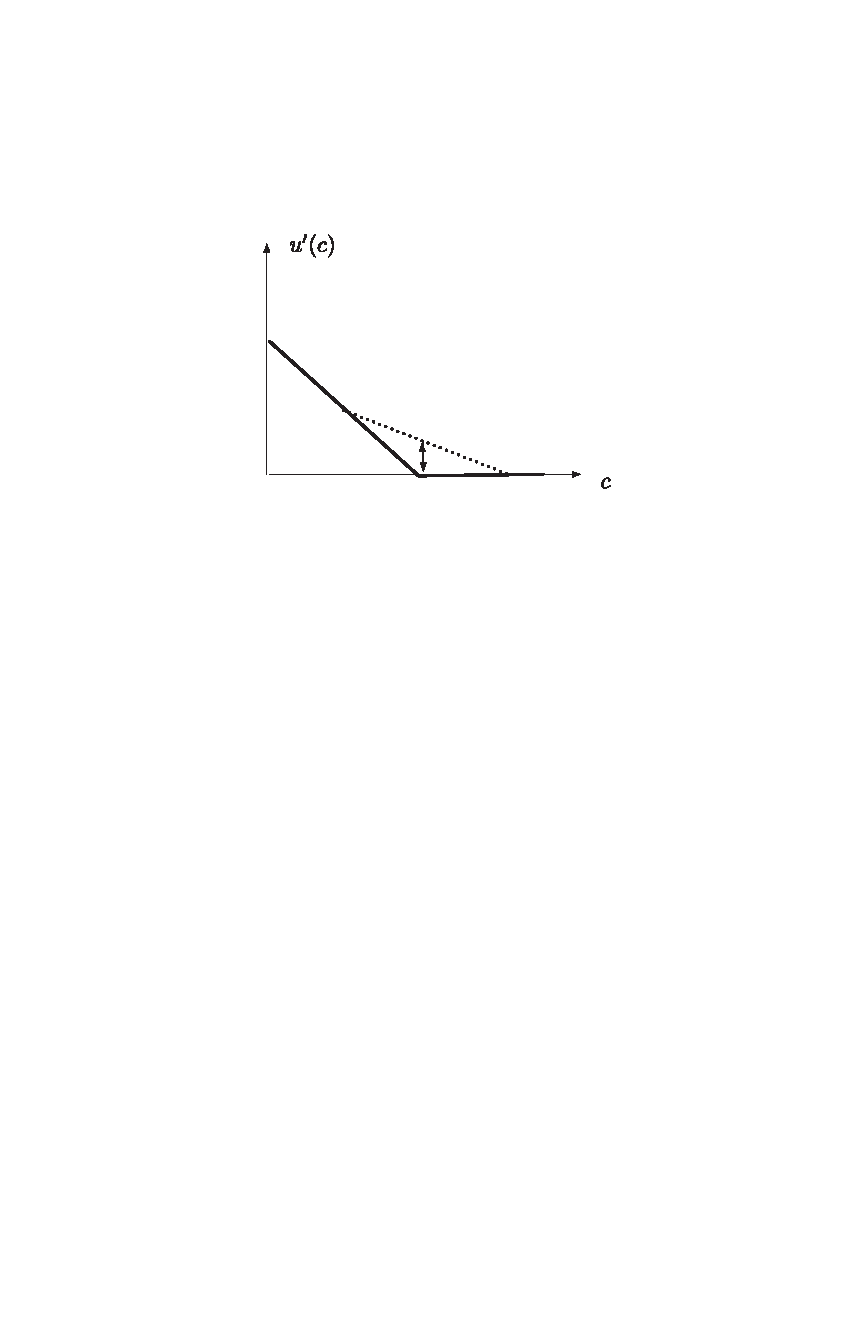
\includegraphics{bagliano.pdf}   }
\end{tabular}
\end{center}}
Convexity of the marginal utility will play an important role for the results below. 

\noindent Taking derivatives with respect to $A_0$, the optimality condition is 



\begin{equation}
U^{\prime}(\frac{a}{b}-A_0)= \frac{1}{2} \underset{\text{Marg. U in bad state}}{\underbrace{U^{\prime}(A_0+\frac{a}{b}-\sigma)}} + \frac{1}{2} \underset{\text{Marg. U in good state}}{\underbrace{U^{\prime}(A_0+\frac{a}{b}+\sigma)}}
\label{euler1}
\end{equation}%




If $\sigma=0$ the first order condition becomes 

\begin{equation}
U^{\prime}(\frac{a}{b}-A_0)=  U^{\prime}(A_0+\frac{a}{b})
\label{2 - CB1}
\end{equation}%

It is immediate that the solution is $A_0=0$, which allows perfect consumption smoothing ($ C_0=C_1=a/b $). Suppose now that there is income risk in the second period. We find the solution following two steps. 


Step 1: We show that when $\sigma>0$, $A_0=0$ is not optimal.  In fact, evaluate  (\ref{euler1}) at $A_0=0$. We show that the foc is not satisfied. The left-hand side in (\ref{euler}) is zero. To see the value of the righ-hand side, notice that when $A_0=0$, in the second period the agent consumes either $\frac{a}{b}+\sigma$ (with zero marginal utility) or $\frac{a}{b}-\sigma$ (with positive marginal utility) with equal probability. Looking at the Figure, the right hand side is strictly positive because marginal utility is convex.  Therefore, the optimality condition is violated. When $\sigma>0$ the agent is induced to save in the first period: $A_0>0$ and $C_0<a/b$, which raises the time-0 marginal utility above zero. 

Step 2: Since  $A_0>0$, we now know that the marginal utility in the good state is zero (because $A_0+\frac{a}{b}+\sigma>a/b$). Recalling that when $C<a/b$ marginal utility is $a-bC$, (\ref{euler1}) becomes

\begin{equation}
a-b(\frac{a}{b}-A_0) =  \frac{1}{2} [a-b (A_0+\frac{a}{b}-\sigma)]
\label{euler}
\end{equation}%

which allows to solve for \begin{equation}A_0= \frac{\sigma}{3} \end{equation}

Then, using the budget constraints
\begin{equation}
C_{0} =\frac{a}{b}-\frac{\sigma}{3} 
\label{2 - CB}
\end{equation}
Consumption in the second period is a random variable: 


\begin{equation}
C_1=\left\{ 
\begin{array}{l}
a/b +\sigma  +   \frac{\sigma}{3} \text{\qquad  } avec  \  \ \ \ probabilite \ 1/2 \\ 
a/b -\sigma +  \frac{\sigma}{3}  \text{\qquad } avec \ probabilite \  1/2  %
\end{array}%
\right.  \label{uti}
\end{equation}



\indent Face au risque, l'agent a tendance a epargner, ce qui abaisse le niveau de consommation courante. The higher $\sigma$ is, the higher $A_0$. The Covid crisis has increased the propensity to save.  See graph, showing a spike in the (declared) propensity to save of French households during and after the spring lockdown. The PIH would predict that facing a temporary negative shock on income, individuals should save less.  So, why has saving propensity increased? Part of the explanation is forced saving: some expenditures were not possible during the lockdown, consumers do not feel confortable travelling, etc. However, part of the explanation is the precautionary motive. In fact, the COVID-19 pandemic has triggered a massive spike in uncertainty (about the the infectiousness of the virus, how long it will take to develop effective vaccines, the economic implications, etc).  

\end{enumerate}

{\samepage
\begin{center}
\begin{tabular}{c}
\resizebox{12cm}{8cm}{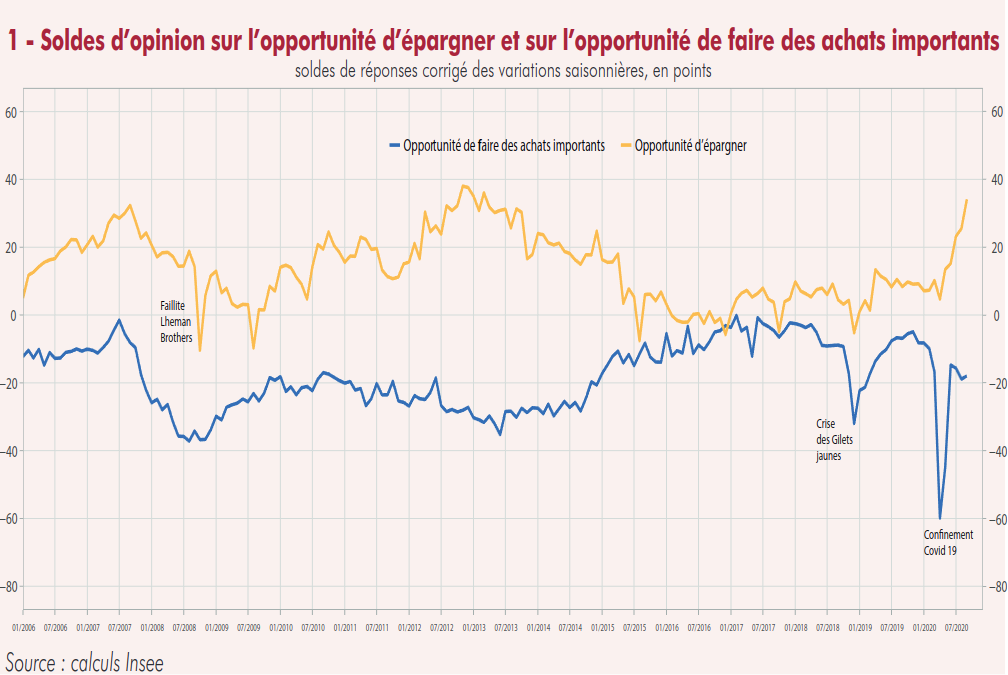
\includegraphics{insee_epargne.pdf}   }
\end{tabular}
\end{center}}


\end{document}
